\documentclass{standalone}
\usepackage{tikz,color}
\begin{document}

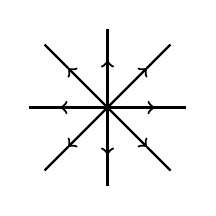
\begin{tikzpicture}
\draw [->,thick] (0,0) to (-0.6,0);
\draw [->,thick] (0,0)  to (0.6,0);
\draw [-,thick ] (-1,0) to (1,0);
\draw [->,thick] (0,0) to (0,0.6);
\draw [->,thick] (0,0)  to (0,-0.6);
\draw [-,thick ] (0,-1) to (0,1);
\draw [->,thick, domain= 0:0.5, samples=25] plot({\x},{\x});
\draw [-,thick, domain=  0.5:0.8, samples=25] plot({\x},{\x});
\draw [->,thick, domain= 0:0.5, samples=25] plot({-\x},{\x});
\draw [-,thick, domain=  0.5:0.8, samples=25] plot({-\x)},{\x});
\draw [->,thick, domain= 0:0.5, samples=25] plot({\x},{-\x});
\draw [-,thick, domain=  0.5:0.8, samples=25] plot({\x},{-\x)});
\draw [->,thick, domain= 0:0.5, samples=25] plot({-\x},{-\x});
\draw [-,thick, domain=  0.5:0.8, samples=25] plot({-\x},{-\x});

\end{tikzpicture}
\end{document}
